\documentclass{article}
\usepackage[bottom=2cm, right=1.5cm, left=1.5cm, top=2cm]{geometry}
\usepackage{amsmath}
\usepackage{amssymb}
\usepackage{amsthm}
\usepackage{enumitem}
\usepackage{exercise} % Exercises Style
\usepackage{graphicx}
\usepackage{caption}
\usepackage{environ}



% Enable Code
\usepackage{minted}
\let \extra T

\newcommand{\vect}[1]{\boldsymbol{#1}}
\DeclareMathOperator{\Tr}{Tr}
\DeclareMathOperator{\Cov}{Cov}
\DeclareMathOperator{\Var}{Var}
\DeclareMathOperator{\E}{E}

\usepackage{fancyhdr}
\newenvironment{solution}
  {\renewcommand\qedsymbol{$\blacksquare$}\begin{proof}[Solution]$ $}
  {\end{proof}}

\title{Solutions to Assignment 8}
\author{Rongfei Jin}
\begin{document}

\pagestyle{fancy}
\fancyhf{}%
\fancyhead[L]{\textbf{ DS5220 \ Assignment 8 }}
\fancyhead[R]{\textbf{Rongfei Jin}}
\fancyfoot[C]{\thepage}%
\maketitle


\section{ISLR}
\subsection{Conceptual 2}
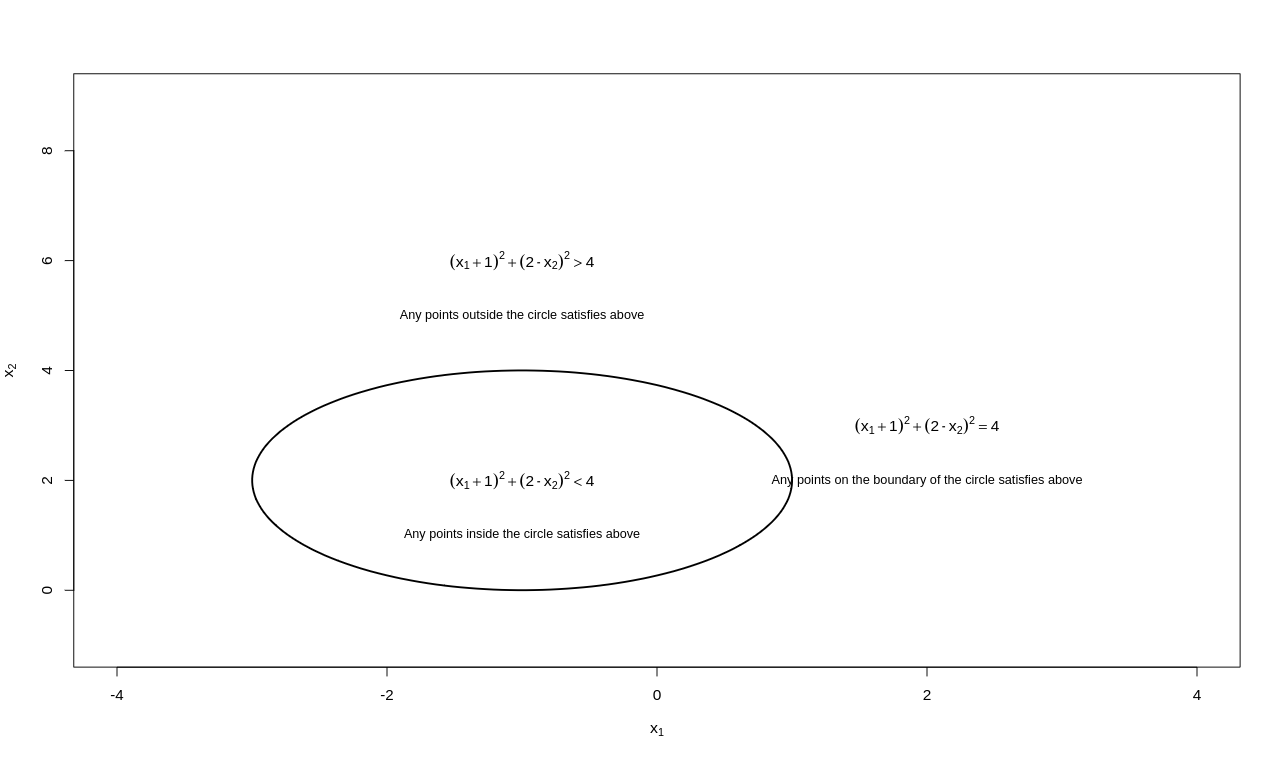
\includegraphics[width=0.75\textwidth]{figs/q2-1.png}
\newline
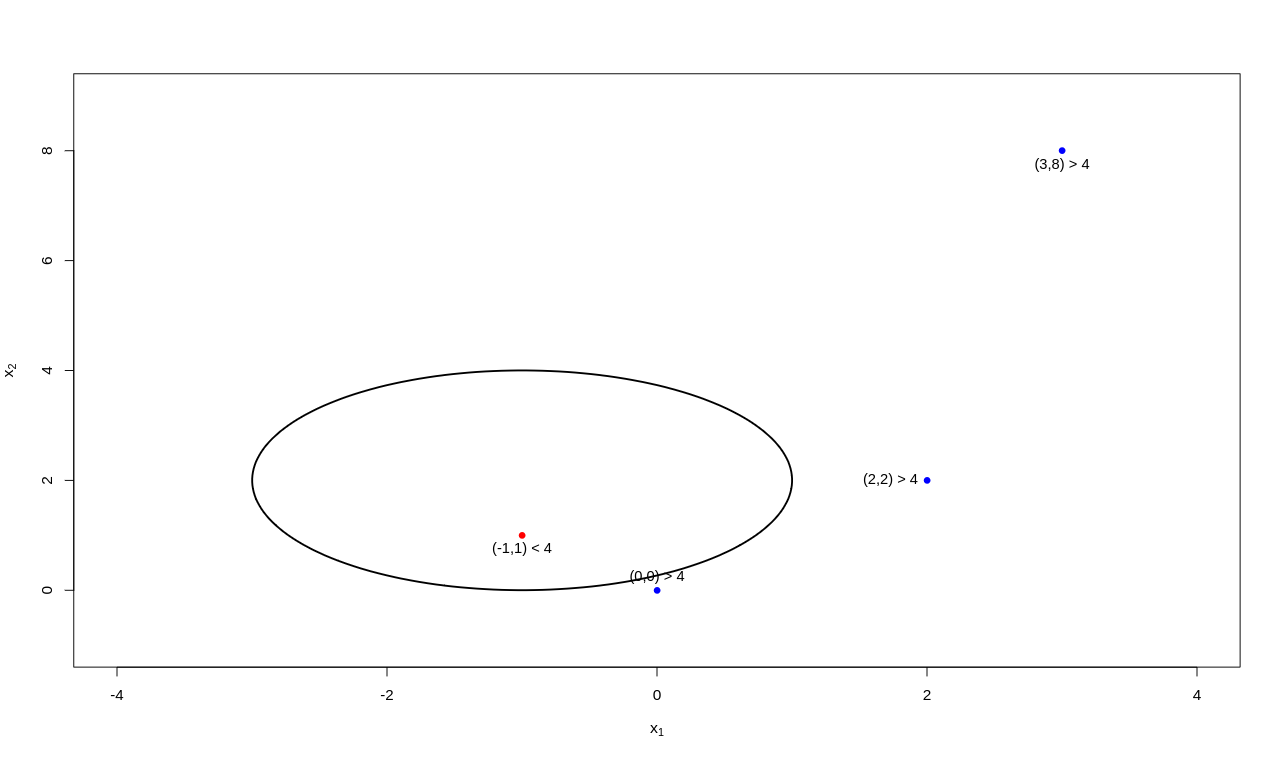
\includegraphics[width=0.75\textwidth]{figs/q2-2.png}

\subsubsection{(d)}
One can expandsn the expression as follow
\begin{align*}
(1+X_1)^2 + (2-X_2) &= 4 \\
1 + 2X_1 + X_1^2 + 4 - 4X_2 + X_2^2 &= 4 \\
1 + 2X_1 + X_1^2 - 4X_2 + X_2^2 &= 0 \\
\end{align*}

The left hand side is not a linear combination of $X_1$ and $X_2$, thus it is not a linear

\newpage
\subsection{Conceptual 3}
\subsubsection*{(a), (d)}

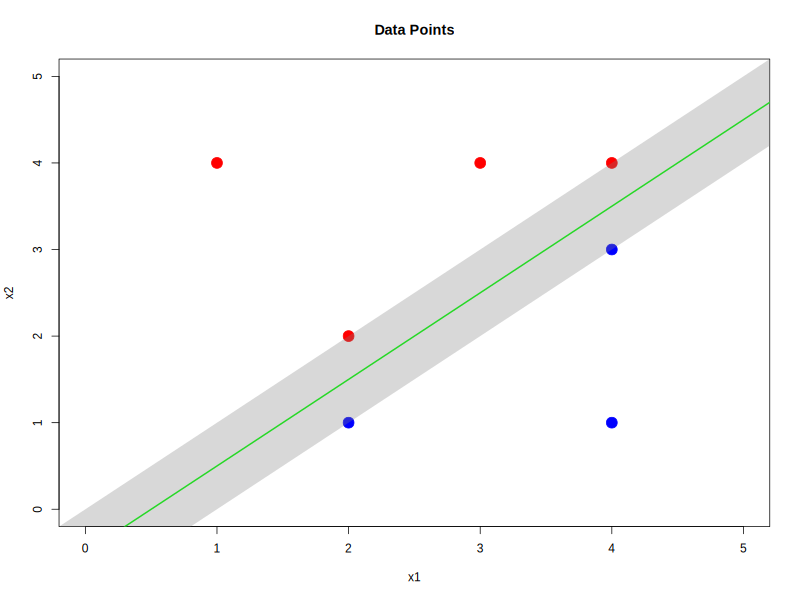
\includegraphics[width=0.75\textwidth]{figs/q3-1.png}
\newline
The width of the gray rectangular region indicates the margin

\subsubsection*{(c), (b)}
The decision boundary is given by \(0.5 + X_1 - X_2 = 0\)

Classifiy to Red if \(0.5 + X_1 - X_2 > 0\), otherwise classify to Blue. 

\subsubsection*{(e)}
The support vectors are (2,1), (2,2), (4,3), (4,4)
\subsubsection*{(f)}
The maximal margin hyperplane is only determined by the support vectors, thus the decision boundary will not change if we slightly move the 7th observation


\subsubsection*{(g)}
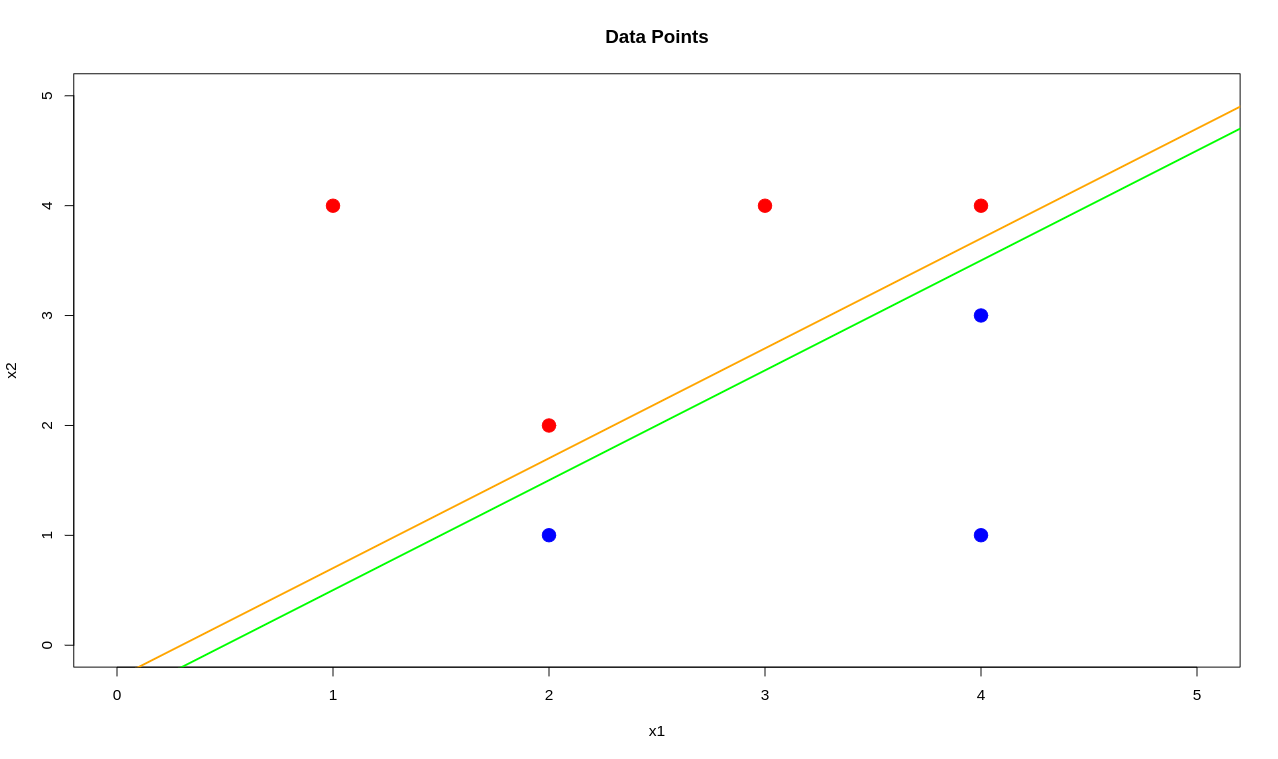
\includegraphics[width=0.75\textwidth]{figs/q3-2.png}
\newline
The orange line is the non-optimal hyperplane
\subsubsection*{(f)}
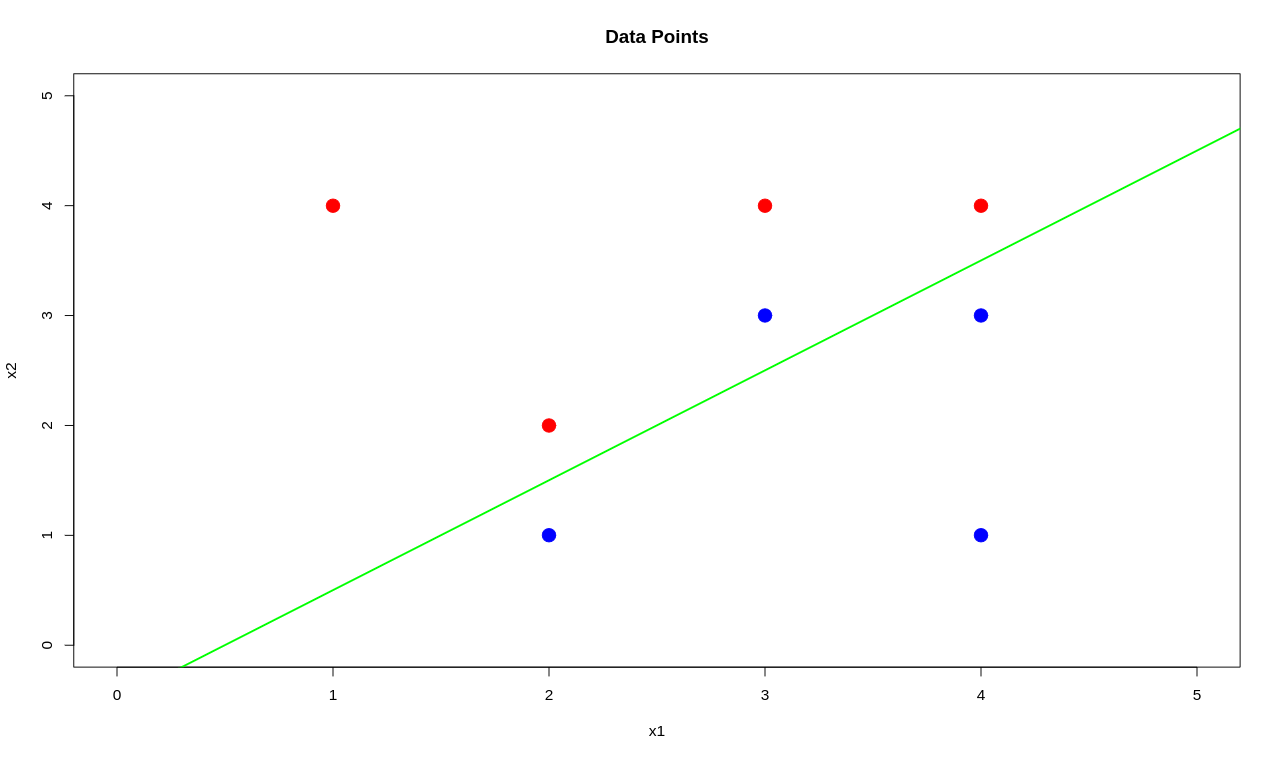
\includegraphics[width=0.75\textwidth]{figs/q3-3.png}

\newpage
\subsection{Applied 5}

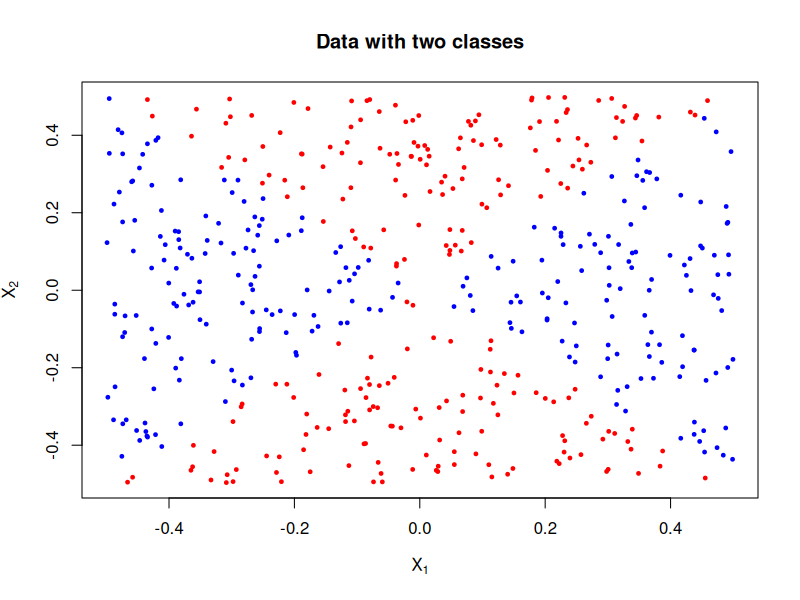
\includegraphics[width=0.75\textwidth]{figs/q5-1.png}
\newline
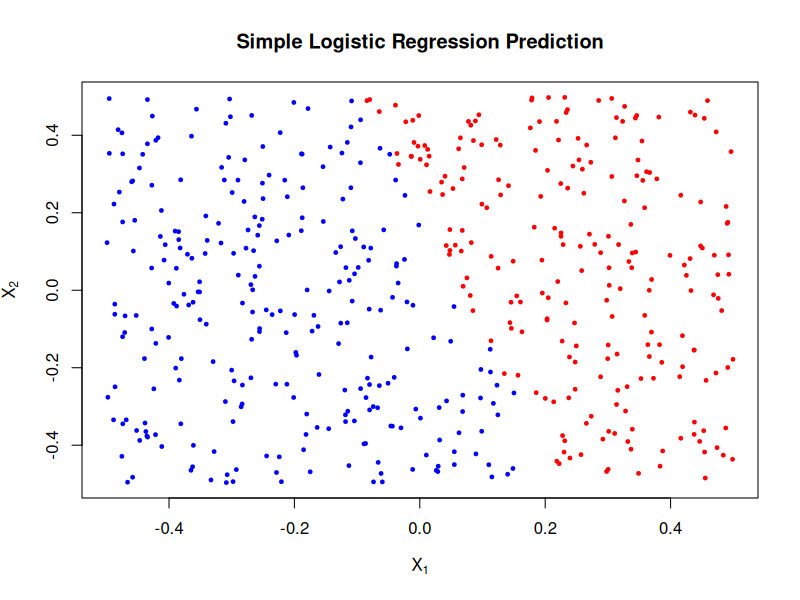
\includegraphics[width=0.75\textwidth]{figs/q5-2.png}
\newline
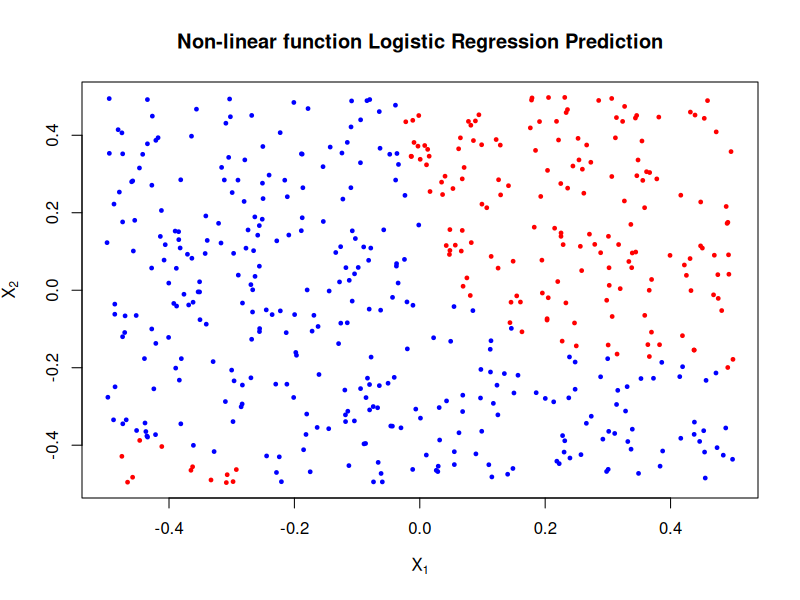
\includegraphics[width=0.75\textwidth]{figs/q5-3.png}
\newline
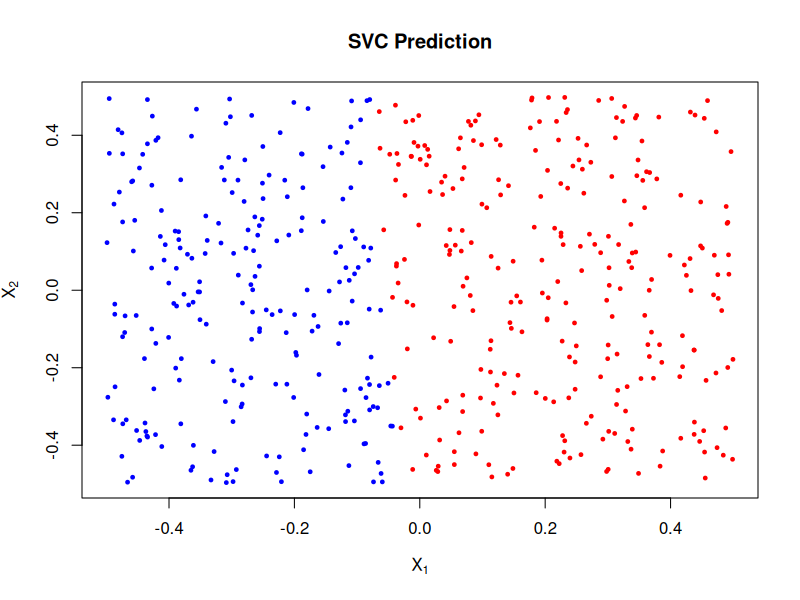
\includegraphics[width=0.75\textwidth]{figs/q5-4.png}
\newline
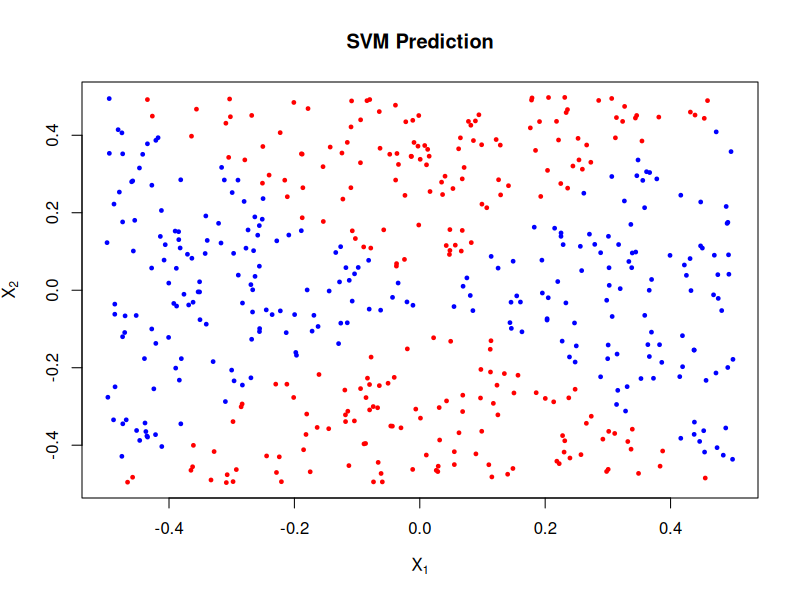
\includegraphics[width=0.75\textwidth]{figs/q5-5.png}
\newline


The logistic regression models, either linear or non-linear feature, are able to classify some of the data, but not all of them. The decision boundary is not optimal as it does not separate the data well.

The SVM with linear kernel is not able to classify the data well, as the data is not linearly separable.

The SVM with radial kernel is able to classify the data well, as it can capture the non-linear relationship between the features.

\inputminted{r}{src/q5.R}
\newpage
\subsection{Applied 8}

Based on the summaries, both radial and polynomial d=2 basi utilized over 630 vectors where the linear models utilized much less vectors around 340.

Based on the test errors the tuned linear model performed the best with 0.15, while the polynomial models performed the worst

\inputminted{r}{src/q8.R}

\newpage
\section{ESL}
\subsection{Ch 4, Exercise 7}
The criterion enforces the value \(\beta^T x_i + \beta_0\) to be the distance to the hyperplane

However, the constraint does not solve the problem because the max margin hyperplane is not necessarily the one that minimizes the distance to the hyperplane.
\subsection{Ch 12, Exercise 1}

\begin{align}
&\underset{\beta, \beta_0}{\min} \frac{1}{2} \|\beta\|^2 + C \sum_{i=1}^n \xi_i \\
&\text{subject to } \xi_i \ge 1-y_i(\beta^T x_i + \beta_0), \quad \xi_i \geq 0, \quad i = 1, \ldots, n
\end{align}


\[
\underset{\beta, \beta_0}{\min} \sum_{i=1}^{N}[1-y_i f(x_i)]_+ + \frac{\lambda}{2} \|\beta\|^2
\]

let \(\lambda = \frac{1}{C}\)
\begin{align}
&\underset{\beta, \beta_0}{\min} \sum_{i=1}^{N}[1-y_i f(x_i)]_+ + \frac{1}{2C} \|\beta\|^2\\
\iff & \underset{\beta, \beta_0}{\min} \frac{1}{2} \|\beta\|^2 + C \sum_{i=1}^n [1-y_i f(x_i)]_+ \\
\end{align}

Now any \(\beta, \beta_0\) that satifies (4) will satisfy (1)

Now consider \(\xi_i > 1 - y_i f(x_i)\) by the KKT conditions we have
\[
a_i[y_i (\beta^T x_i + \beta_0) - (1- \xi_i)] = 0
\]

\[\mu_i = 0\]

Since \(\xi_i > 1 - y_i f(x_i)\) we have \(a_i = 0\)

\[
L_p = \frac{1}{2} \|\beta\|^2 + C \sum_{i=1}^n \xi_i - \sum_{i=1}^{N}\mu_i \xi_i - \sum_{i=1}^{N} a_i [1-y_i f(x_i) - \xi_i]
\]
Therefore the primal function minimization problem above is equivalent to (1)

\end{document}